\chapter{Temo: Sistemo de Lindenmayer}

{ }\hfill\textbf{Nivelo:} Alta

Por ^ci tiu parto, mi indiku kelkajn refera^jojn:
\begin{itemize}
 \item de la retpa^go Vikipedio pri la L-sistemoj: \texttt{http://eo.wikipedia.org/wiki/L-Sistemo}.
 \item de la libro \og The Algorithmic Beauty of Plants\fg{} verkita
   de Przemyslaw Prusinkiewicz kaj Aristid Lindenmayer.
\end{itemize}

\vspace*{0.5cm} 

Temos pri la nocio de sistemo de Lindenmayer a^u L-sistemo inventita
en 1968 de la biologo hungaro Aristid Lindenmayer.  L-Sistemo estas
aro da reguloj kaj simboloj kiuj modelas procezon de kreskado de
vivuloj kiel plantoj a^u ^celoj.  La ^cefa koncepto de la L-sistemoj
estas la nocio de reskribado.  Reskribado estas te^hniko por konstrui
malsimplajn objektojn per anstata^uigi partojn de komenca simpla
objekto uzante regulojn de reskribado.

Por fari tion, la ^celoj estas modelitaj per simboloj.  Je ^ciu
generacio, la ^celoj disparti^gas, tio estas, simbolon anstata^uas unu
a^u pluraj aliaj simboloj formantaj vorton.

\section{Formala difino}

L-sistemo estas formala gramatiko konsistanta el:
\begin{enumerate}
\item Unu alfabeto $V$: l' aro de la variabloj de la L-Sistemo. $V *$
  estas la aro de la ``vortoj'' kiujn oni povas konstrui per la simboloj
  de $V$, kaj $V +$ l' aro de la vortoj enhavantaj almena^u unu simbolon.
\item Unu aro de valoroj konstantaj $S$.  Kelkaj el tiuj simboloj
  estas komunaj al ^ciuj L-Sistemoj (^cefe kiam uzi la testudon).
\item Unu komenca aksiomo $\omega$ elektita inter $V +$ , tio estas la
  komenca stato.
\item Unu ekzemplo de reguloj, indikata $P$, pri reproduktado de la
  simboloj de $V$.
\end{enumerate}

L-sistemo estas do indikata $\{V,S,\omega,P\}$.

Konsideru la jenan L-sistemon:
\begin{itemize}
\item Alfabeto: $V = \{A, B\}$
\item Konstantoj: $S = \{\emptyset\}$
\item Komenca aksiomo: $\omega = A$
\item Reguloj: 
  $\begin{array}{|l|}
    \hline
    A \rightarrow AB \\
    B \rightarrow A \\ 
    \hline
  \end{array}$
\end{itemize}
La du reguloj donitaj estas la reguloj de reskribado de la sistemo.
Je ^ciu stadio, $A$ estas anstata^uita de la sinsekvo $AB$, kaj $B$
estas anstata^uita de $A$.  Jen la unuaj iteracioj de tiu sistemo de
Lindemayer:
\begin{center}
  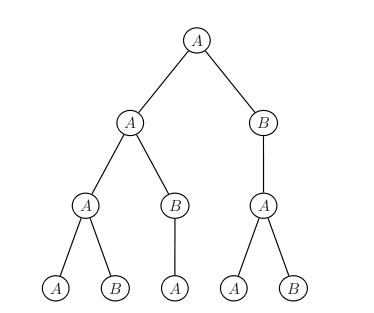
\includegraphics[width=8cm]{bildoj/linden-arbre.png}
\end{center}
\begin{itemize}
\item Iteracio 1: $A$
\item Iteracio 2: $AB$
\item Iteracio 3: $ABA$
\item Iteracio 4: $ABAAB$
\end{itemize}
\vspace*{0.2cm}
Bone, bone... sed konkrete? Da^urigu legi!

\section{Interpretado de la testudo}

Tiu unua ekzemplo ebligis vin kompreni la nocion de sistemo de
Lindenmayer, eble sen ekkonscii kiel ni uzos tion konkrete kun la
testudo.

Ja tie tio esti^gas interesa: ^Ciu vorto tiel konstruita nur havas
propran signifon.  Oni tiam kro^cos al ^ciu litero de la sinsekvo,
komandon rulotan de la testudo, por tiel generi desegnojn 2D a^u 3D.

\subsection{Oftaj simboloj}
\begin{itemize}
 \item [\textbullet] $F$ : Movi^gi je unu unueca pa^so ($\in V$)
 \item [\textbullet] $+$ : Turni^gi maldekstren je angulo $\alpha$ $(\in S)$.
 \item [\textbullet] $-$ : Turni^gi dekstren je angulo $\alpha$ $(\in S)$.
 \item [\textbullet] $\&$ : Pivoti al malsupro je angulo $\alpha$ $(\in S)$.
 \item [\textbullet] \textasciicircum : Pivoti al supro je angulo $\alpha$ $(\in S)$.
 \item [\textbullet] \textbackslash: Ruli^gi maldekstren je angulo $\alpha$ $(\in S)$.
 \item [\textbullet] $/$: Ruli^gi dekstren je angulo $\alpha$ $(\in S)$.
 \item [\textbullet] $|$: Efektivigi duonturni^gon.  En XLogo: \texttt{dn 180}
\end{itemize}
\vspace*{0.2cm}
Ni prenu por ekzemplo $\alpha=90$ kaj unuecan movi^gon je $10$ testudpa^sojn; jen:
\begin{center}
 \begin{tabular}{|c|c|c|c|c|c|c|c|c|}
 \hline
Simbolo & $F$ & $+$ & $-$ & $\&$ & \textasciicircum & \textbackslash& $/$ & $|$ \\
 \hline
Komando XLogo & \texttt{an 10}&\texttt{mdn 90}&\texttt{dn 90}&\texttt{malsupren 90}&\texttt{supren 90}&\texttt{mdfn 90}&\texttt{dfn 90}&\texttt{dn 180}\\
 \hline
\end{tabular}
\end{center}
\subsection{Ne^gero de Koch}
Konsideru la L-sistemon:
\begin{itemize}
 \item [\textbullet] Komenca stato: $F--F--F--$
 \item [\textbullet] Produkta regulo: $F \rightarrow F+F--F+F$
 \item [\textbullet] Angulo $\alpha=60$\degre, la unuecan pa^son oni dividu per $3$ 
   je ^ciu iteracio.
\end{itemize}
Unuaj iteracioj:
\begin{center}
\begin{minipage}{7.5cm}
 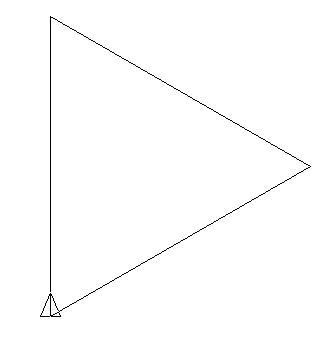
\includegraphics[width=7.5cm]{bildoj/linden-flocon1.png}
\end{minipage}
\begin{minipage}{7.5cm}
 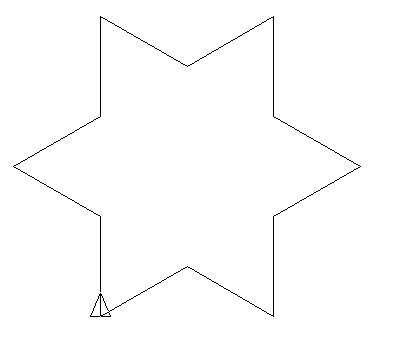
\includegraphics[width=7.5cm]{bildoj/linden-flocon2.png}
\end{minipage}\\
\begin{minipage}{7.5cm}
 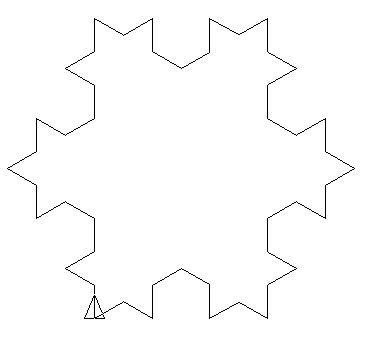
\includegraphics[width=7.5cm]{bildoj/linden-flocon3.png}
\end{minipage}
\begin{minipage}{7.5cm}
 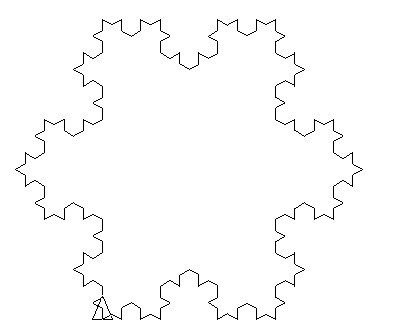
\includegraphics[width=7.5cm]{bildoj/linden-flocon4.png}
\end{minipage}
\end{center}
Programo en Logo:
\begin{verbatim}
por neĝero :p
provizu "unuo 300 / potencon 3 :p-1
ripetu 3 [F :p-1 td 120]  
fino

por F :p
se :p=0 [an :unuo haltu]
F :p-1 mdn 60 F :p-1 dn 120 F :p-1 md 60
F :p-1 
fino
\end{verbatim}

\subsection{Kurbo de Koch je ordo 2}
Ni interesi^gu pri la jena L-sistemo:
\begin{itemize}
 \item[\textbullet] Komenca stato: $F-F-F-F$
 \item[\textbullet] Produkta regulo: $F\rightarrow F-F+F+FF-F-F+F$
\end{itemize}

Jen la unuaj reprezentoj uzante $\alpha=90$ kaj alĝustigante la unuecan pa^son tiel ke
la figuro havu ^ciam la saman amplekson:
\begin{center}
\begin{minipage}{7.5cm}
 
\includegraphics[width=7.5cm]{bildoj/linden-koch1.png}
\end{minipage}
\begin{minipage}{7.5cm}
 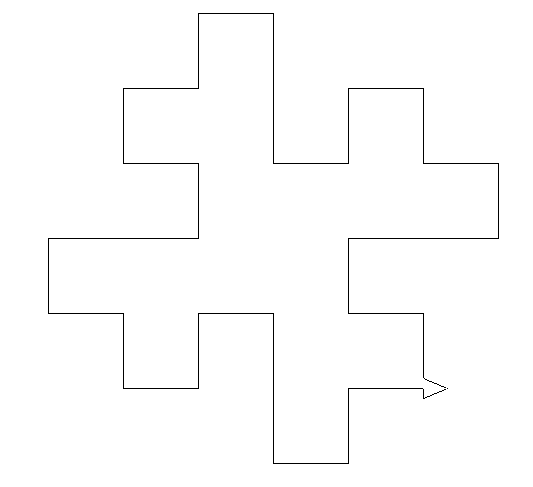
\includegraphics[width=7.5cm]{bildoj/linden-koch2.png}
\end{minipage}\\
\begin{minipage}{7.5cm}
 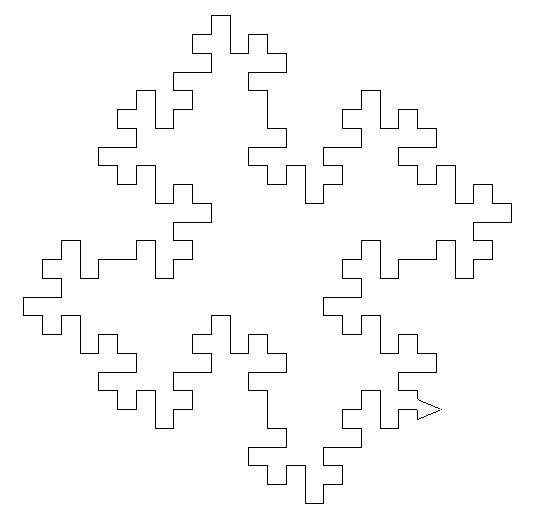
\includegraphics[width=7.5cm]{bildoj/linden-koch3.png}
\end{minipage}
\begin{minipage}{7.5cm}
 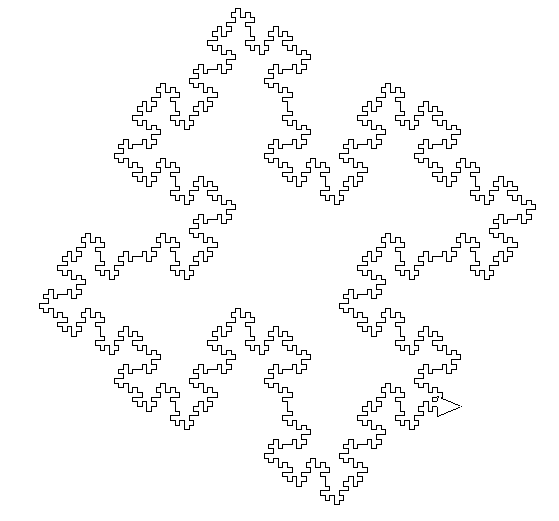
\includegraphics[width=7.5cm]{bildoj/linden-koch4.png}
\end{minipage}
\end{center}
Tre facilas do krei la programon Logo ebligantan generi tiujn desegnojn:
\begin{verbatim}
# p indikas l' iteracion
por koch :p
  # Je ĉiu iteracio, la unueca distanco dividatas per 4
  # Ĉi tie, la fina figuro havos amplekson 600x600 maksimume
  provizu "unuo 300 / potencon 4 :p-1
  ripetu 3 [F :p-1 tg 90] F :p-1 
fino

# La ĉeno reskribada
por F :p
  se :p=0 [an :unuo haltu]
  F :p-1 mdn 90 F :p-1 dn 90 F :p-1 dn 90
  F :p-1 F :p-1 mdn 90 F :p-1 mdn 90 F :p-1 dn 90 F :p-1
fino
\end{verbatim}

\subsection{Kurbo de l' dragono}
\begin{itemize}
 \item[\textbullet] Komenca stato: $F$\\
 \item[\textbullet] Produkta regulo: $\begin{array}{|l|}
\hline
A\rightarrow A+B+ \\
B\rightarrow -A-B \\
\hline
\end{array}$ 
\end{itemize}
\begin{verbatim}
por a :p
se :p=0 [an :unuo haltu]
a :p-1 mdn 90 b :p-1 mdn 90
fino

por b :p
se :p=0 [an :unuo haltu]
dn 90 a :p-1 dn 90 b :p-1
fino

por dragono :p
provizu "unuo 300 / 8 / :p  
a :p
fino
\end{verbatim}
\begin{center}
 \begin{minipage}{7cm}
 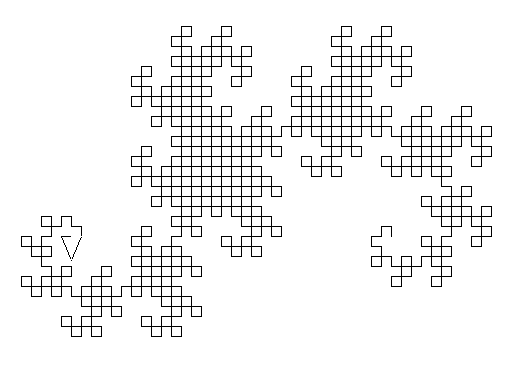
\includegraphics[width=7cm]{bildoj/linden-dragon10.png}
 \begin{center}
  \texttt{dragono 10}
 \end{center}
\end{minipage}
 \begin{minipage}{7cm}
 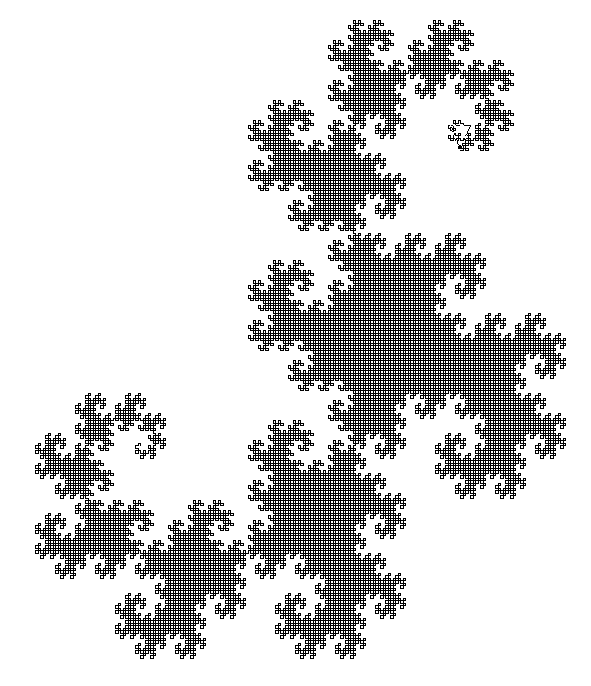
\includegraphics[width=7cm]{bildoj/linden-dragon15.png}
 \begin{center}
  \texttt{dragono 15}
 \end{center}
\end{minipage}
\end{center}

\subsection {Kurbo de Hilbert en 3D}

La sekva ekzemplo estas la kurbo de Hilbert en la spaco; ^gi estas
kurbo kun la atributo plenigi tute kubon kiam oni pligrandigas la
nombron de iteracioj .

Jen la rilata sistemo:
\begin{itemize}
 \item Komenca stato: $A$
 \item Angulo $\alpha=90$\degre, dividu la unuecan longon per du je
   ^ciu iteracio.
 \item Produkta regulo: 
   $\begin{array}{|l|}
     \hline
     A\rightarrow B-F+CFC+F-D\&F \textrm{\textrm{\textasciicircum}} D-F+\&\&CFC+F+B// \\
     B\rightarrow A\&F\textrm{\textrm{\textasciicircum}} CFB\textrm{\textasciicircum} F 
     \textrm{\textasciicircum} D\textrm{\textasciicircum} \textrm{\textasciicircum}-F-D
     \textrm{\textasciicircum}|F\textrm{\textasciicircum} B|FC\textrm{\textasciicircum} 
     F\textrm{\textasciicircum} A// \\
     C\rightarrow|D\textrm{\textasciicircum}|F\textrm{\textasciicircum} B-F+C\textrm{\textasciicircum} 
     F\textrm{\textasciicircum} A\&\&FA\&F\textrm{\textasciicircum} C+F+B\textrm{\textasciicircum} F
     \textrm{\textasciicircum} D// \\
     D\rightarrow|CFB-F+B|FA\&F\textrm{\textasciicircum} A\&\&FB-F+B|FC// \\
     \hline
   \end{array}$
\end{itemize}
\begin{verbatim}
por hilbert :p
ev perspektive
provizu "unuo 400 / potencon 2 :p
linia_difino sdikp :unuo/2
a :p
linia_difinhalto
tridimensie_vidigu
fino

por a :p
se :p=0 [haltu]
b :p-1 dn 90 an :unuo mdn 90 c :p-1 an :unuo c :p-1
mdn 90 an :unuo dn 90 d :p-1 malsupren 90 an :unuo supren 90 d :p-1
dn 90 an :unuo mdn 90 malsupren 180 c :p-1 an :unuo c :p-1
mdn 90 an :unuo mdn 90 b :p-1 dfn 180
fino

por b :p
se :p=0 [haltu]
a :p-1 malsupren 90 an :unuo supren 90 c :p-1 an :unuo b :p-1 supren 90 
an :unuo supren 90 d :p-1 supren 180 dn 90 an :unuo dn 90 d :p-1 supren 90 
dn 180 an :unuo supren 90 b :p-1 dn 180 an :unuo c :p-1 supren 90 an :unuo
supren 90 a :p-1 dfn 180 
fino

por c :p
se :p=0 [haltu]
dn 180 d :p-1 supren 90 dn 180 an :unuo supren 90 b :p-1 dn 90 an :unuo mdn 90 
c :p-1 supren 90 an :unuo supren 90 a :p-1 malsupren 180 an :unuo a :p-1 malsupren 90 
an :unuo supren 90 c :p-1 mdn 90 an :unuo mdn 90 b :p-1 supren 90 an :unuo supren 90 
d :p-1 dfn 180 
fino

por d :p
se :p=0 [haltu]
dn 180 c :p-1 an :unuo b :p-1 dn 90 an :unuo mdn 90 b :p-1 dn 180
an :unuo a :p-1 malsupren 90 an :unuo supren 90 a :p-1 malsupren 180 an :unuo
b :p-1 dn 90 an :unuo mdn 90 b :p-1 dn 180 an :unuo c :p-1 dfn 180
fino
\end{verbatim}
Jen l' unuaj iteracioj:
\begin{center}
\begin{minipage}{7cm}
 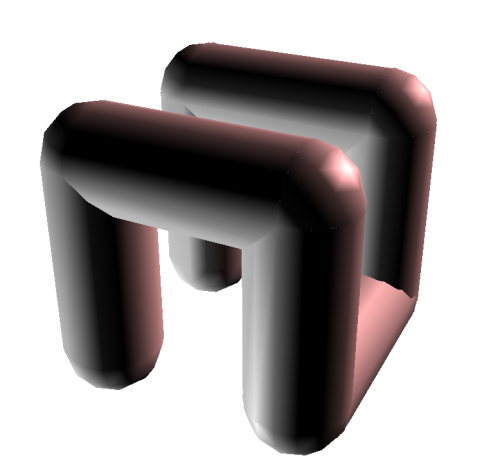
\includegraphics[width=7cm]{bildoj/linden-hilbert1.png}
\end{minipage}
\begin{minipage}{7cm}
 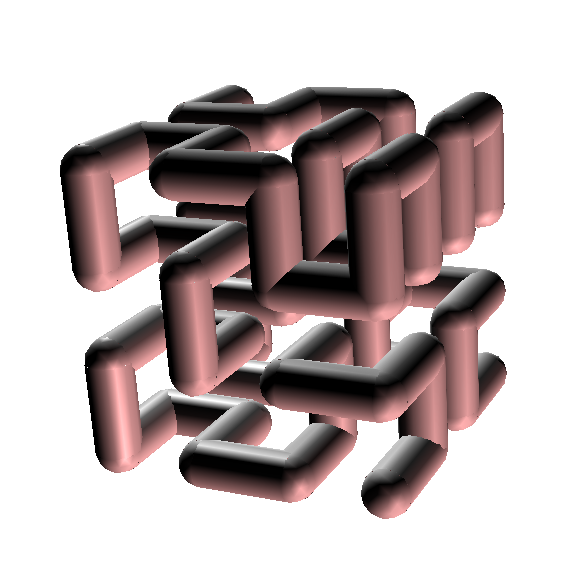
\includegraphics[width=7.5cm]{bildoj/linden-hilbert2.png}
\end{minipage}\\
\begin{minipage}{7cm}
 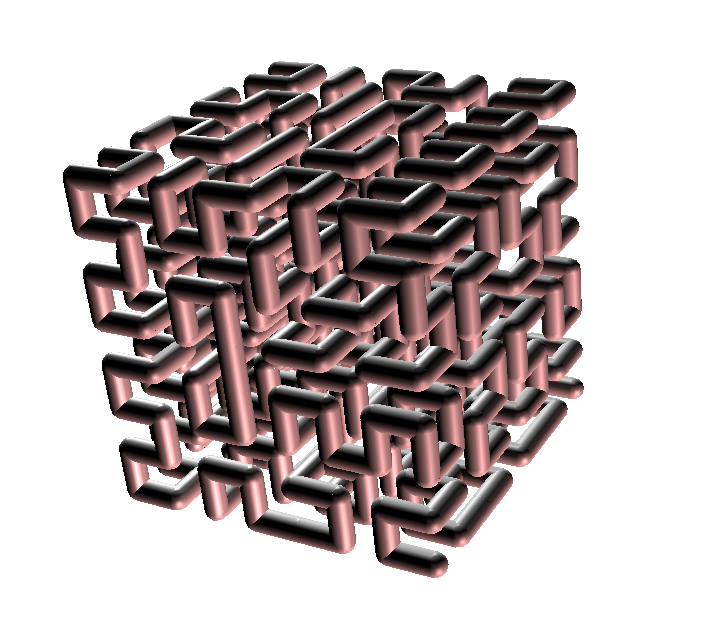
\includegraphics[width=7cm]{bildoj/linden-hilbert3.png}
\end{minipage}
\begin{minipage}{7cm}
 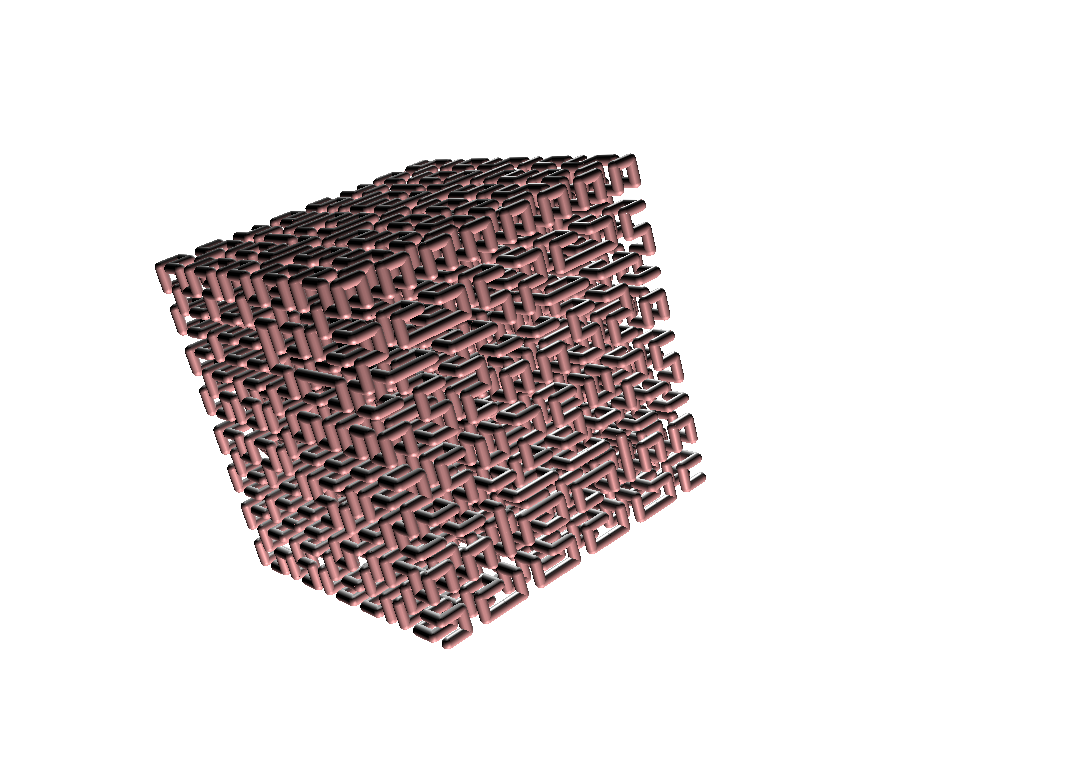
\includegraphics[width=9cm]{bildoj/linden-hilbert4.png}
\end{minipage}
\end{center}
